%! Author = melek
%! Date = 9.06.2022

% Preamble
\documentclass[11pt]{article}

% Packages
\usepackage{amsmath}
\DeclareMathOperator*{\argmax}{argmax}

\usepackage{graphicx}
\usepackage{amssymb}
\usepackage{bm}

\graphicspath{ {../images/} }


% Document
\begin{document}

    \maketitle
    \setcounter{section}{9}


    \section{Exercises}

    \subsection{Question}

    We have not explicitly considered or given pseudocode for any Monte Carlo methods or in this chapter.
    What would they be like?
    Why is it reasonable not to give pseudocode for them?
    How would they perform on the Mountain Car task?

    \subsection*{Answer}

    Monte Carlo method is just an extreme case of n-step methods.
    One can achieve MC effect by using a sufficiently large n value.

    MC is slower to learn.
    MC cannot start learning before an episode ends.

    \subsection{Question}

    Give pseudocode for semi-gradient one-step Expected Sarsa for control.

    \subsection*{Answer}

    We are already given a pseudocode for semi-gradient one-step sarsa control.
    Sarsa update target can be replaced with expected sarsa update target.

    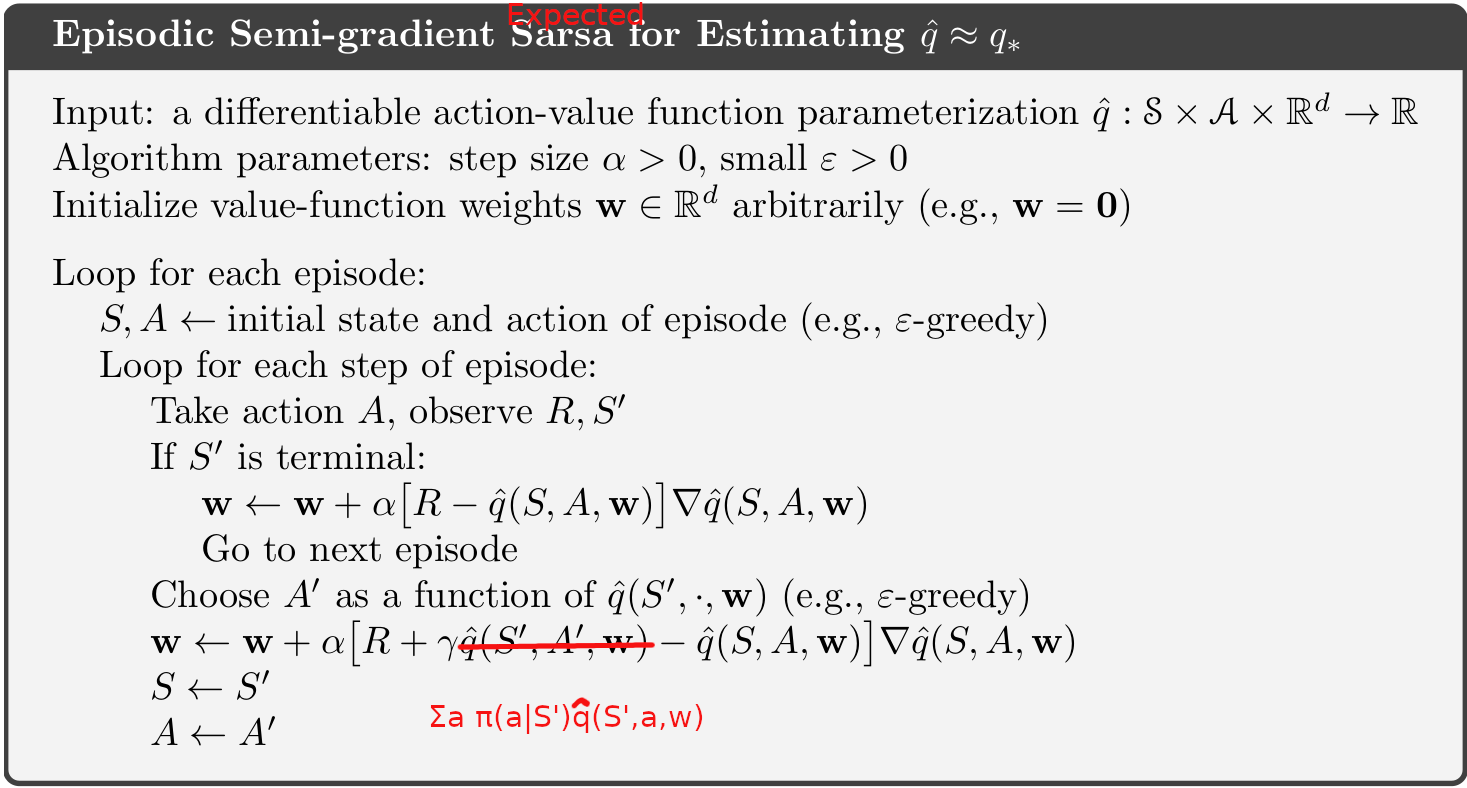
\includegraphics[scale=0.7]{exercise_10_2}

    \subsection{Question}

    Why do the results shown in Figure 10.4 have higher standard errors at large n than at small n?

    \subsection*{Answer}

    The answer is similar to TD methods vs MC methods debate.

    In n-step learning, intermediate values of n works best.
    n-values less than the optimum n value, tends to behave like TD(0) while n-values larger than the optimum n value, tends to behave like MC.

    MC method updates are known to be high variance due to large number of steps thus large number of noise involved.

   \subsection{Question}

    Give pseudocode for a differential version of semi-gradient Q-learning.

    \subsection*{Answer}

    We are already given a pseudocode for a differential version of semi-gradient sarsa.
    Sarsa update target can be replaced with expected q-learning update target.

    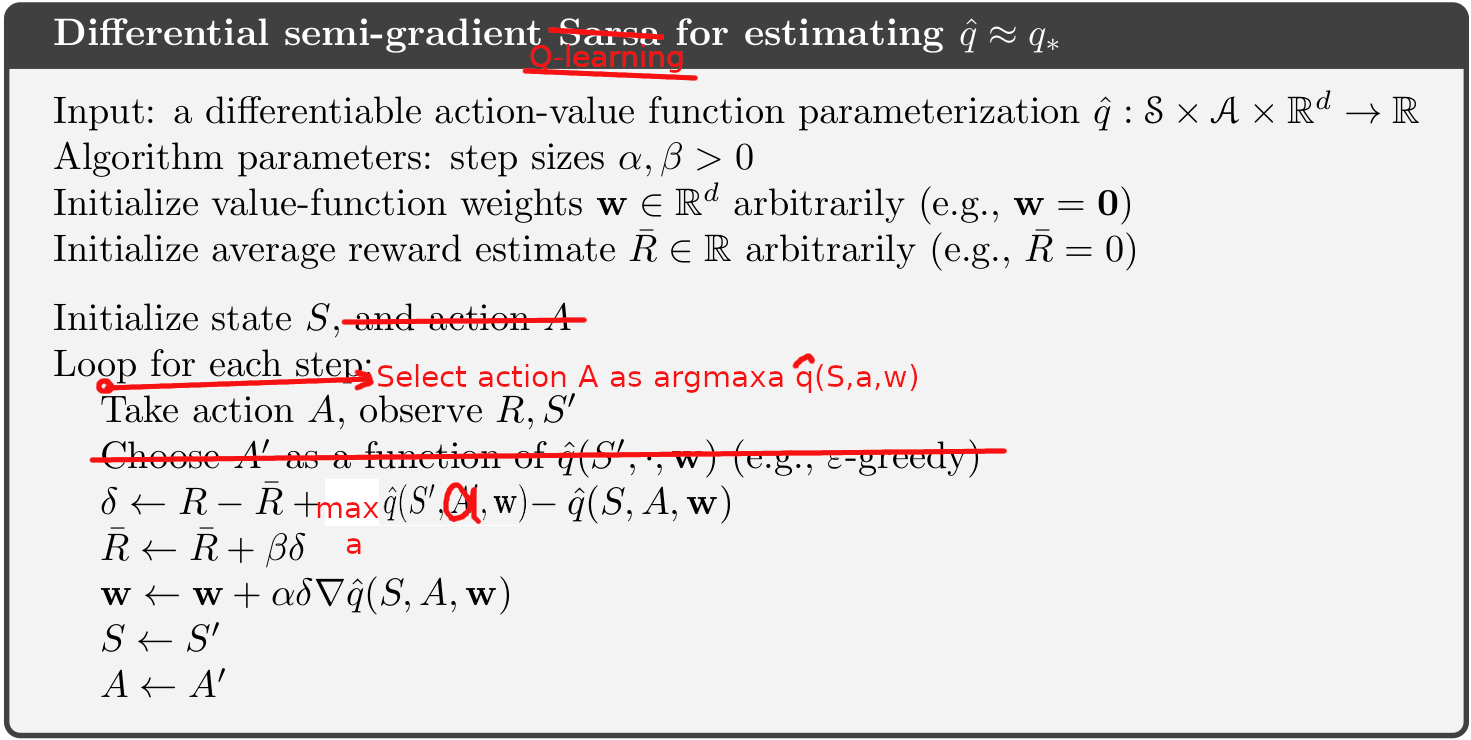
\includegraphics[scale=0.7]{exercise_10_4}

    \subsection{Question}

    What equations are needed (beyond 10.10) to specify the differential version of TD(0)?

    \subsection*{Answer}

    10.10 gives differential form of the two TD errors.
    10.12 gives the average reward version of semi-gradient Sarsa.
    We can leverage those two equations to obtain differential version of TD(0).

    $ w_{t+1} = w_t + \alpha \delta_t \Delta \hat{V}(S_t,w_t) $

    \subsection{Question}

    Consider a Markov reward process consisting of a ring of three states A, B,and C, with state transitions going deterministically around the ring.
    A reward of +1 is received upon arrival in A and otherwise the reward is 0.
    What are the differential values of the three states?

    \subsection*{Answer}

    Ring of 3 states.

   \textbf{A} \rightarrow0\rightarrow \textbf{B} \rightarrow0\rightarrow \textbf{C} \rightarrow+1\rightarrow \textbf{A}

    \noindent Average reward as per 10.7:

    $ r(\pi) = \sum_{s} \mu_{\pi}(s) \sum_{a} \pi(a|s) \sum_{s',r}{p(s',r|s,a)} r $

    $ r(\pi) = 1/3 * 1.0 * 1.0 * 0 + 1/3 * 1.0 * 1.0 * 0 + 1/3 * 1.0 * 1.0 * 1 = 1/3 $

    \noindent State values as per 10.9+:

    $ v_\pi(s) = \sum_{a} \pi(a|s) \sum_{s',r}{p(s',r|s,a)} [r - r(\pi) + v_\pi(s') ] $

    $ v_\pi(A) =  0 - 1/3 + v_\pi(B) = v_\pi(B) - 1/3 $

    $ v_\pi(B) =  0 - 1/3 + v_\pi(C) = v_\pi(C) - 1/3 $

    $ v_\pi(C) =  1 - 1/3 + v_\pi(A) = v_\pi(A) + 2/3 $

    \noindent Linear equations turns out to have many solutions e.g. a plane:
    Let's pick up a value for state B from availability space as $V(B) = 0$.
    Then:

    $V(A) = -1/3$

    $V(C) = 1/3$

    \subsection{Question}

    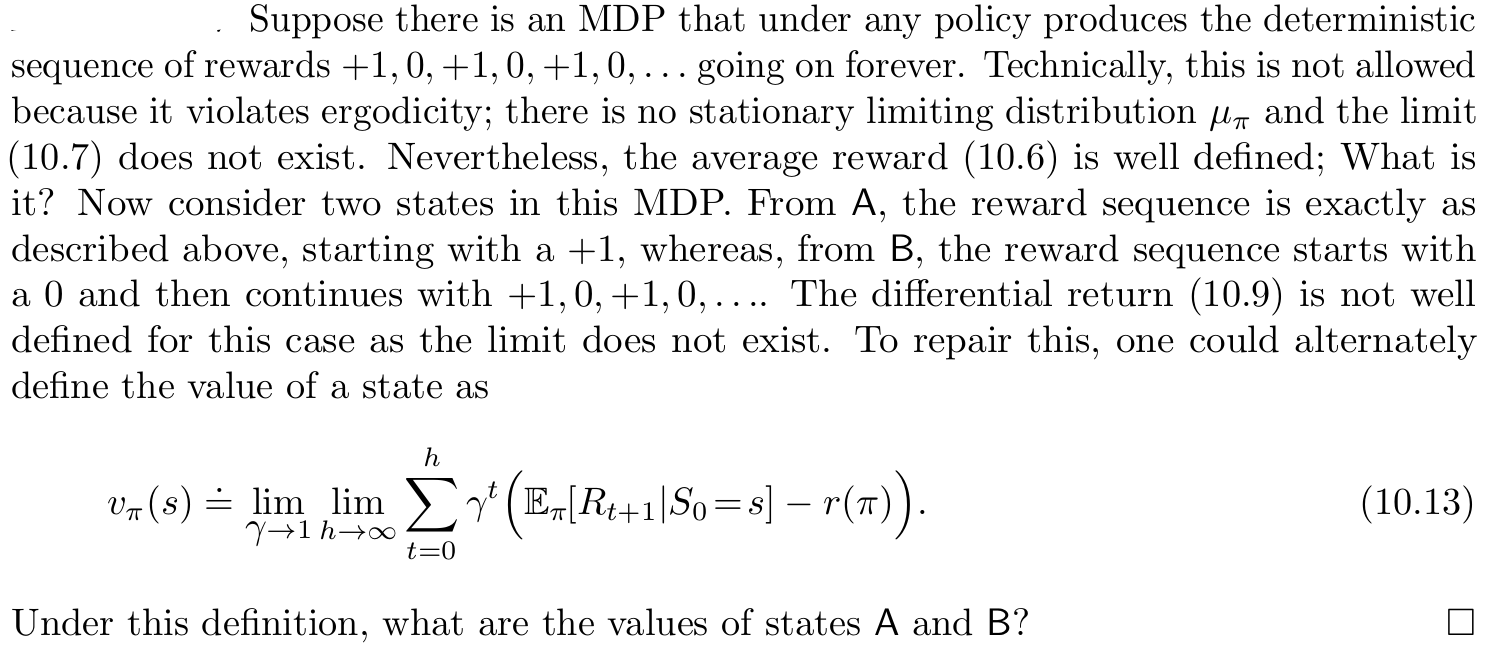
\includegraphics[scale=0.9]{exercise_10_7q}

    \subsection*{Answer}

    \noindent Average reward as per 10.6:

    \noindent $ r(\pi) = \lim_{h \to \infty} \frac{1}{h} \sum_{t=1}^{h} E[R_t |S_0,A_0 \pi] $

    \noindent $ r(\pi) = \lim_{h \to \infty} \frac{1}{h} \sum_{t=1}^{h/2} E[R_{2t-1} |S_0,A_0 \pi] + E[R_{2t} |S_0,A_0 \pi] $

    \noindent $ r(\pi) = \lim_{h \to \infty} \frac{1}{h} \sum_{t=1}^{h/2} 1 + 0 $

    \noindent $ r(\pi) = \lim_{h \to \infty} \frac{1}{h} \frac{h}{2} = 0.5 $

    \noindent Now consider two states in this MDP, as per 10.13:

    \noindent $ v_\pi(s) = \lim_{\gamma \to 1} \lim_{h \to \infty} \sum_{t=0}^{h} \gamma^t (E[R_{t+1} |S_0=s] - r(\pi)) $

    \noindent $ v_\pi(A) = \lim_{\gamma \to 1} \lim_{h \to \infty} \sum_{t=0}^{h} \gamma^t (E[R_{t+1} |S_0=A] - r(\pi)) $

    \noindent $ v_\pi(A) = \lim_{\gamma \to 1} \lim_{h \to \infty} \sum_{t=0}^{h/2} \gamma^{2t} (E[R_{2t+1} |S_0=A] - r(\pi)) + \gamma^{2t+1} (E[R_{2t+2} |S_0=A] - r(\pi)) $

    \noindent $ v_\pi(A) = \lim_{\gamma \to 1} \lim_{h \to \infty} \sum_{t=0}^{h/2} \gamma^{2t} 0.5 + \gamma^{2t+1} (-0.5) $

    \noindent $ v_\pi(A) = \lim_{\gamma \to 1} \lim_{h \to \infty} \sum_{t=0}^{h/2} \gamma^{2t} 0.5  (1-\gamma) $

    \noindent $ v_\pi(A) = \lim_{\gamma \to 1} \lim_{h \to \infty} 0.5  (1-\gamma) \sum_{t=0}^{h/2} \gamma^{2t}  $

     \noindent $ v_\pi(A) = \lim_{\gamma \to 1} \lim_{h \to \infty} 0.5  (1-\gamma) \sum_{t=0}^{h/2} (\gamma^{2})^t  $

    \noindent there we have a geometric series of form $ \frac{1-x^{n+1}}{1-x} = \sum_{k=0}^{n} x^k $

    \noindent $ v_\pi(A) = \lim_{\gamma \to 1} \lim_{h \to \infty} 0.5  (1-\gamma) \frac{1-(\gamma^2)^{h/2+1}}{1-\gamma^2}  $

    \noindent We have $ \lim_{h \to \infty} (\gamma^2)^{h/2+1} = \gamma^{\inf} = 0 $

    \noindent $ v_\pi(A) = \lim_{\gamma \to 1} 0.5  (1-\gamma) \frac{1}{1-\gamma^2}  $

    \noindent $ v_\pi(A) = \lim_{\gamma \to 1} 0.5 \frac{1}{1+\gamma}  $

    \noindent $ v_\pi(A) = 0.5 \frac{1}{2} = 0.25  $

    Calculation for state B is similar:

    \noindent $ v_\pi(B) = \lim_{\gamma \to 1} \lim_{h \to \infty} \sum_{t=0}^{h/2} \gamma^{2t} (E[R_{2t+1} |S_0=A] - r(\pi)) + \gamma^{2t+1} (E[R_{2t+2} |S_0=A] - r(\pi)) $

    \noindent $ v_\pi(B) = \lim_{\gamma \to 1} \lim_{h \to \infty} \sum_{t=0}^{h/2} \gamma^{2t} (-0.5) + \gamma^{2t+1} 0.5 $

    \noindent $ v_\pi(B) = \lim_{\gamma \to 1} \lim_{h \to \infty} -1 \sum_{t=0}^{h/2} \gamma^{2t} 0.5 - \gamma^{2t+1} 0.5 $

    \noindent Which makes:

    \noindent $ v_\pi(B) = -1 v_\pi(A)  = -0.25 $


    \subsection{Question}

    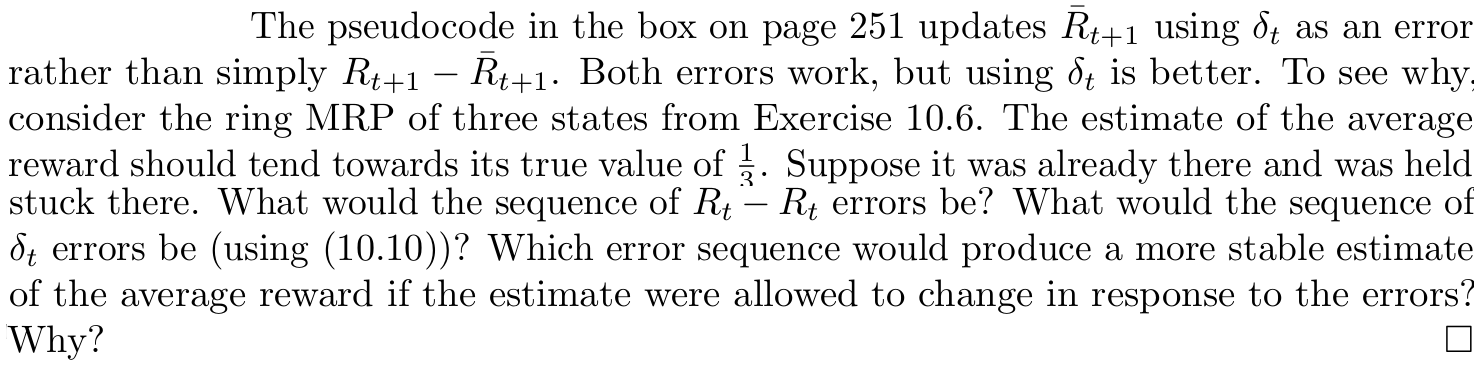
\includegraphics[scale=0.9]{exercise_10_8q}

    \subsection*{Answer}

    Using state values from 10.6.
    v(A) = -1/3,
    v(B) = 0,
    v(C) = 1/3.

    \noindent Average reword $ \bar{R}=\frac{1}{3} $ as given in the question.

    \hfill \break
    \noindent Let's calculate average reward using 10.10 after each state transition.

    \noindent $ \delta = R - \bar{R} + \hat{q}(S',A',w) - \hat{q}(S',A,w) $
    \noindent $  \bar{R} = \bar{R} + \beta \delta $

    \noindent State A, transition to state B

    \noindent $ \delta = 0 - \frac{1}{3} + 0 - (-\frac{1}{3}) = 0 $

    \noindent State B, transition to state C

    \noindent $ \delta = 0 - \frac{1}{3} + \frac{1}{3} - 0 = 0 $

    \noindent State C, transition to state A

    \noindent $ \delta = 1 - \frac{1}{3} + (-\frac{1}{3}) - \frac{1}{3} = 0 $

    \hfill \break
    \noindent If we were to use the simpler update, then update amounts would be:

    \noindent State A, transition to state B

    \noindent $ R - \bar{R} = 0 - \frac{1}{3} = -\frac{1}{3} $

    \noindent State B, transition to state C

    \noindent $ R - \bar{R} = 0 - \frac{1}{3} = -\frac{1}{3} $

    \noindent State C, transition to state A

    \noindent $ R - \bar{R} = 1 - \frac{1}{3} = \frac{2}{3}$

    \hfill \break
    The simpler update rule changes what was supposed to be true value of the average reward.
    TD error does not change the average reward.
    Thus TD error based update produce a more stable estimate.
    Because the simpler update rule does not care about convergence of the average reward.
    TD error based update rule on the other hand slows down if close to convergence.

    \subsection{Question}

    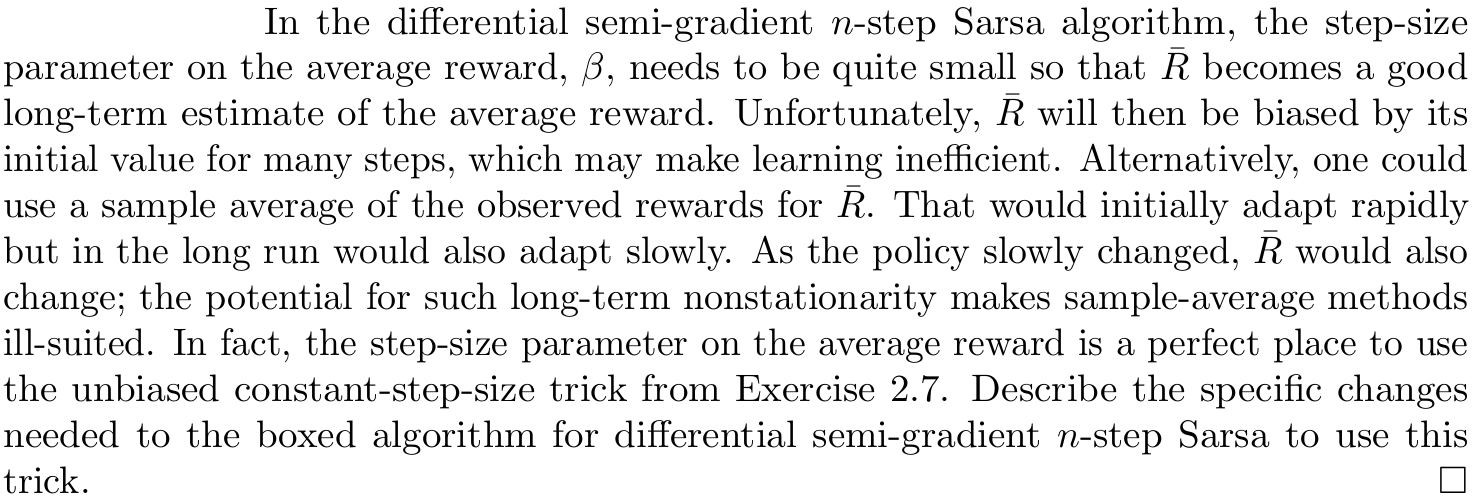
\includegraphics[scale=0.9]{exercise_10_9q}

    \subsection*{Answer}

    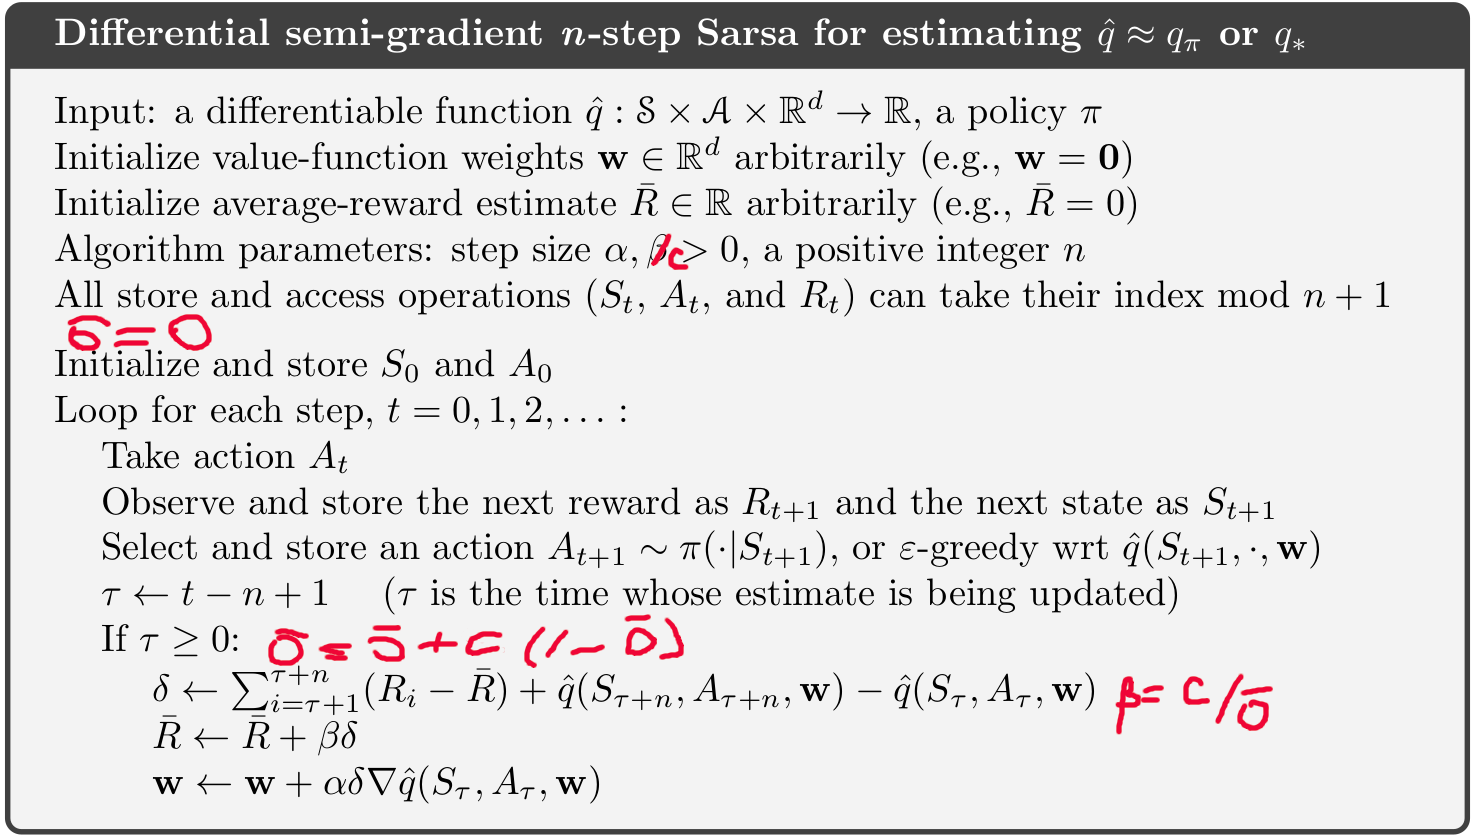
\includegraphics[scale=0.8]{exercise_10_9}
\end{document}


